\documentclass[tikz,border=12pt]{standalone}
\usepackage[T1]{fontenc}
\usepackage{tgheros}
\usepackage{sfmath}
\usepackage{amsmath}
\usepackage{amssymb}
% % \usepackage{fontawesome5} (Removed for publication-grade academic typography) (Removed for publication-grade academic typography)
\usepackage{tikz}
\usetikzlibrary{arrows.meta,positioning,shapes.geometric,fit,backgrounds,calc}
\usepackage{xcolor}

\renewcommand{\familydefault}{\sfdefault}

% Academic Semantic Palette
\definecolor{harvardcrimson}{HTML}{A51C30}
\definecolor{ethdarkblue}{HTML}{1F407A}
\definecolor{ethblue}{HTML}{215CAF}
\definecolor{ethpetrol}{HTML}{007A87}
\definecolor{ethbronze}{HTML}{B87333}
\definecolor{ethpurple}{HTML}{5B4B8A}
\definecolor{ethslate}{HTML}{475569}
\definecolor{cardbg}{HTML}{F8FAFC}
\definecolor{cardborder}{HTML}{CBD5E1}

\definecolor{boxbluebg}{HTML}{EFF6FF}
\definecolor{boxblueborder}{HTML}{3B82F6}
\definecolor{boxtealbg}{HTML}{ECFDF5}
\definecolor{boxtealborder}{HTML}{10B981}
\definecolor{boxamberbg}{HTML}{FFFBEB}
\definecolor{boxamberborder}{HTML}{F59E0B}
\definecolor{boxpurplebg}{HTML}{F5F3FF}
\definecolor{boxpurpleborder}{HTML}{8B5CF6}

\begin{document}
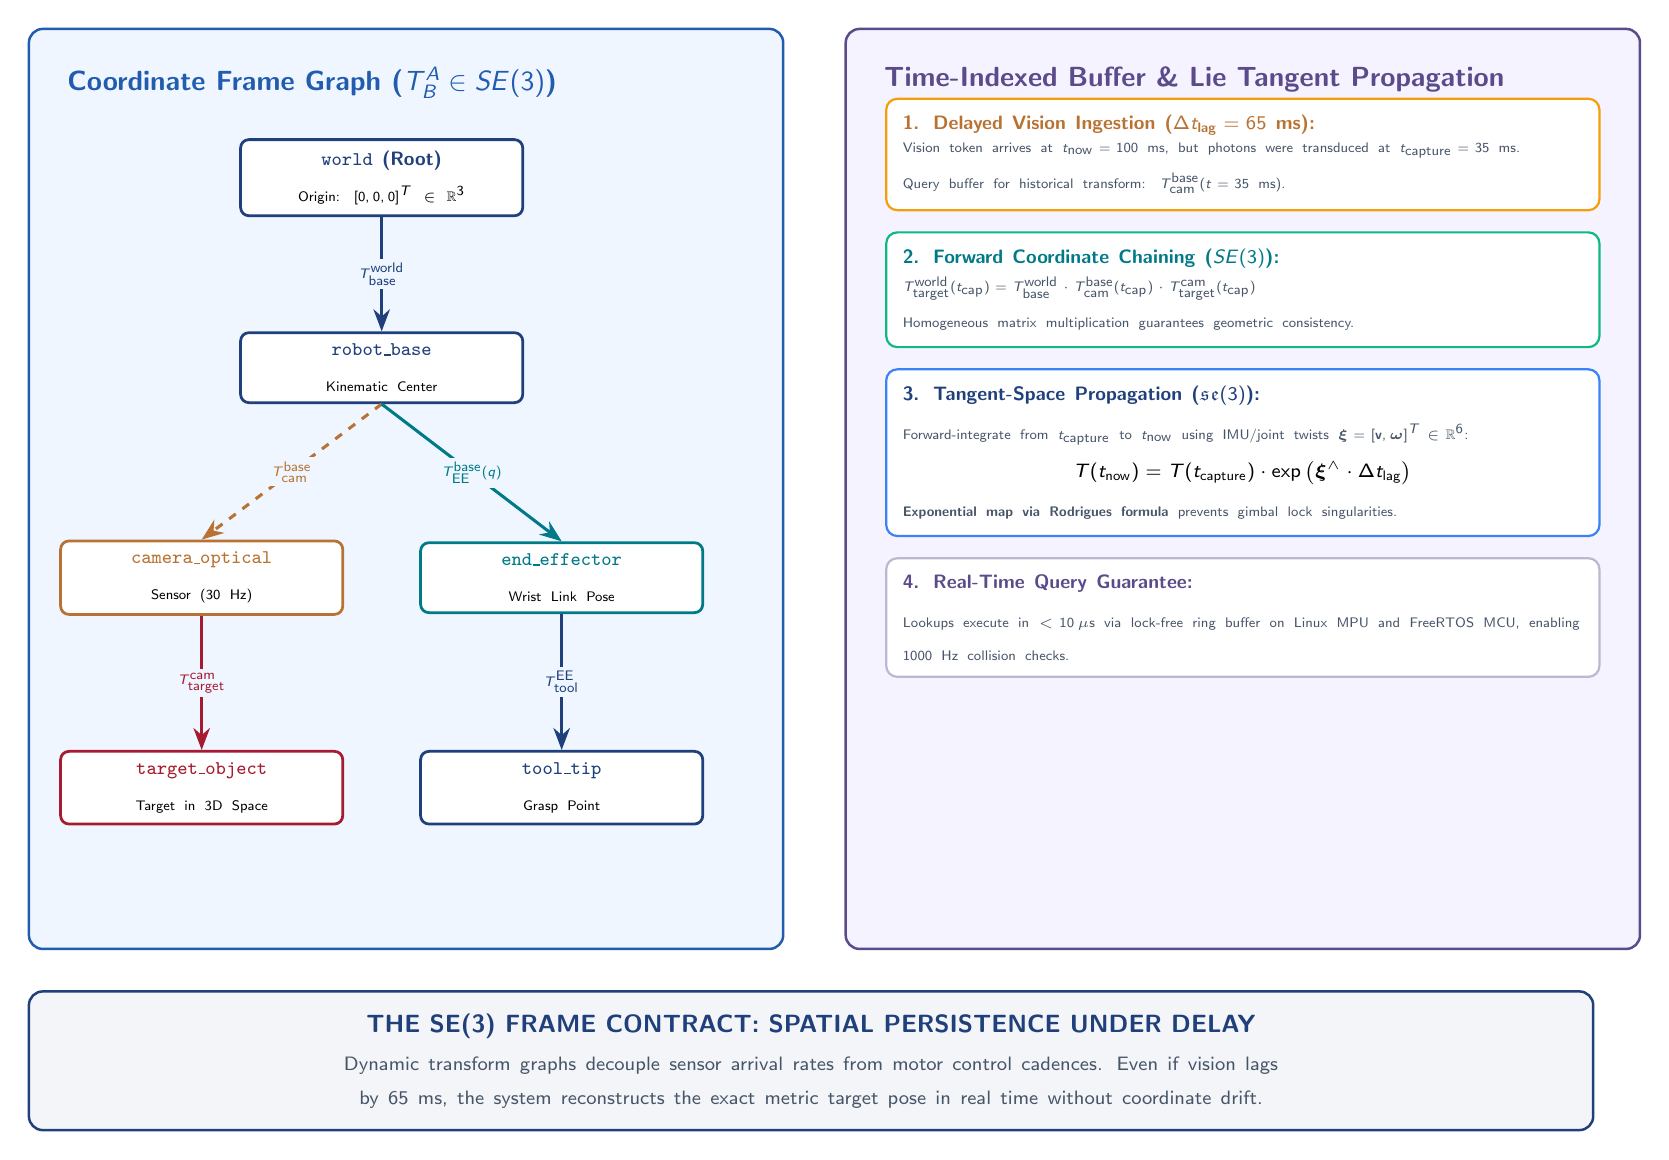
\begin{tikzpicture}[
  font=\sffamily,
  >=Stealth,
  card/.style={
    draw=cardborder,
    fill=white,
    rounded corners=5pt,
    line width=0.9pt,
    inner sep=8pt,
    align=center
  },
  treenode/.style={
    draw=#1,
    fill=white,
    rounded corners=3pt,
    line width=1pt,
    inner sep=4pt,
    text width=1.30in,
    align=center
  },
  stepcard/.style={
    draw=#1,
    fill=white,
    rounded corners=4pt,
    line width=0.8pt,
    inner sep=6pt,
    text width=3.40in,
    align=left
  }
]

  % --- LEFT REGION: FRAME GRAPH HIERARCHY ---
  \node[card, draw=ethblue, fill=boxbluebg, text width=3.55in, minimum height=4.60in, anchor=north west] (treecard) at (0, 0) {};
  \node[anchor=north west, font=\bfseries\color{ethblue}] at ($(treecard.north west)+(0.15in, -0.15in)$) {Coordinate Frame Graph ($T_B^A \in SE(3)$)};

  % Tree Nodes
  \node[treenode=ethdarkblue] (world) at ($(treecard.north west)+(1.77in, -0.75in)$) {
    {\scriptsize\bfseries\color{ethdarkblue} \texttt{world} (Root)}\\[1pt]
    {\tiny Origin: $[0, 0, 0]^T \in \mathbb{R}^3$}
  };

  \node[treenode=ethdarkblue] (robot_base) at ($(world)+(0, -0.95in)$) {
    {\scriptsize\bfseries\color{ethdarkblue} \texttt{robot\_base}}\\[1pt]
    {\tiny Kinematic Center}
  };

  \node[treenode=ethbronze] (camera_optical) at ($(robot_base)+(-0.90in, -1.05in)$) {
    {\scriptsize\bfseries\color{ethbronze} \texttt{camera\_optical}}\\[1pt]
    {\tiny Sensor ($30\text{ Hz}$)}
  };

  \node[treenode=harvardcrimson] (target_object) at ($(camera_optical)+(0, -1.05in)$) {
    {\scriptsize\bfseries\color{harvardcrimson} \texttt{target\_object}}\\[1pt]
    {\tiny Target in 3D Space}
  };

  \node[treenode=ethpetrol] (end_effector) at ($(robot_base)+(0.90in, -1.05in)$) {
    {\scriptsize\bfseries\color{ethpetrol} \texttt{end\_effector}}\\[1pt]
    {\tiny Wrist Link Pose}
  };

  \node[treenode=ethdarkblue] (tool_tip) at ($(end_effector)+(0, -1.05in)$) {
    {\scriptsize\bfseries\color{ethdarkblue} \texttt{tool\_tip}}\\[1pt]
    {\tiny Grasp Point}
  };

  % Connecting Directed Arrows with Edge Labels
  \draw[->, line width=1.1pt, ethdarkblue] (world.south) -- (robot_base.north)
    node[midway, fill=boxbluebg, inner sep=1.5pt, font=\tiny\color{ethslate}] {$T_{\text{base}}^{\text{world}}$};

  \draw[->, line width=1.1pt, ethbronze, dashed] (robot_base.south) -- (camera_optical.north)
    node[midway, fill=boxbluebg, inner sep=1.5pt, font=\tiny\color{ethbronze}] {$T_{\text{cam}}^{\text{base}}$};

  \draw[->, line width=1.1pt, harvardcrimson] (camera_optical.south) -- (target_object.north)
    node[midway, fill=boxbluebg, inner sep=1.5pt, font=\tiny\color{harvardcrimson}] {$T_{\text{target}}^{\text{cam}}$};

  \draw[->, line width=1.1pt, ethpetrol] (robot_base.south) -- (end_effector.north)
    node[midway, fill=boxbluebg, inner sep=1.5pt, font=\tiny\color{ethpetrol}] {$T_{\text{EE}}^{\text{base}}(q)$};

  \draw[->, line width=1.1pt, ethdarkblue] (end_effector.south) -- (tool_tip.north)
    node[midway, fill=boxbluebg, inner sep=1.5pt, font=\tiny\color{ethdarkblue}] {$T_{\text{tool}}^{\text{EE}}$};

  % --- RIGHT REGION: TEMPORAL BUFFER & LIE ALGEBRA INTEGRATION ---
  \node[card, draw=ethpurple, fill=boxpurplebg, text width=3.75in, minimum height=4.60in, right=0.30in of treecard.north east, anchor=north west] (buffercard) {};
  \node[anchor=north west, font=\bfseries\color{ethpurple}] at ($(buffercard.north west)+(0.15in, -0.15in)$) {Time-Indexed Buffer \& Lie Tangent Propagation};

  \node[stepcard=boxamberborder, below=0.35in of buffercard.north] (s1) {
    {\scriptsize\bfseries\color{ethbronze} 1. Delayed Vision Ingestion ($\Delta t_{\text{lag}} = 65\text{ ms}$):}\\[2pt]
    {\tiny\color{ethslate}Vision token arrives at $t_{\text{now}} = 100\text{ ms}$, but photons were transduced at $t_{\text{capture}} = 35\text{ ms}$.\\[1pt]Query buffer for historical transform: $T_{\text{cam}}^{\text{base}}(t=35\text{ ms})$.}
  };

  \node[stepcard=boxtealborder, below=0.10in of s1] (s2) {
    {\scriptsize\bfseries\color{ethpetrol} 2. Forward Coordinate Chaining ($SE(3)$):}\\[2pt]
    {\tiny\color{ethslate}$T_{\text{target}}^{\text{world}}(t_{\text{cap}}) = T_{\text{base}}^{\text{world}} \cdot T_{\text{cam}}^{\text{base}}(t_{\text{cap}}) \cdot T_{\text{target}}^{\text{cam}}(t_{\text{cap}})$\\[1pt]Homogeneous matrix multiplication guarantees geometric consistency.}
  };

  \node[stepcard=boxblueborder, below=0.10in of s2] (s3) {
    {\scriptsize\bfseries\color{ethdarkblue} 3. Tangent-Space Propagation ($\mathfrak{se}(3)$):}\\[2pt]
    {\tiny\color{ethslate}Forward-integrate from $t_{\text{capture}}$ to $t_{\text{now}}$ using IMU/joint twists $\boldsymbol{\xi} = [\mathbf{v}, \boldsymbol{\omega}]^T \in \mathbb{R}^6$:}\\[2pt]
    \centering{\scriptsize $T(t_{\text{now}}) = T(t_{\text{capture}}) \cdot \exp\left(\boldsymbol{\xi}^\wedge \cdot \Delta t_{\text{lag}}\right)$}\\[2pt]
    \raggedright{\tiny\color{ethslate}\textbf{Exponential map via Rodrigues formula} prevents gimbal lock singularities.}
  };

  \node[stepcard=ethpurple!40, below=0.10in of s3] (s4) {
    {\scriptsize\bfseries\color{ethpurple} 4. Real-Time Query Guarantee:}\\[2pt]
    {\tiny\color{ethslate}Lookups execute in $< 10\,\mu\text{s}$ via lock-free ring buffer on Linux MPU and FreeRTOS MCU, enabling $1000\text{ Hz}$ collision checks.}
  };

  % Bottom Synthesis Banner
  \node[card, draw=ethdarkblue, fill=ethdarkblue!5, text width=7.60in, below=0.20in of treecard.south west, anchor=north west] (footer) {
    {\small\bfseries\color{ethdarkblue} THE SE(3) FRAME CONTRACT: SPATIAL PERSISTENCE UNDER DELAY}\\[2pt]
    {\scriptsize\color{ethslate}Dynamic transform graphs decouple sensor arrival rates from motor control cadences. Even if vision lags by $65\text{ ms}$, the system reconstructs the exact metric target pose in real time without coordinate drift.}
  };

\end{tikzpicture}
\end{document}
